\chapter{State of the Art}
\label{cap:estadoDeLaCuestion}

\section{Gmail API}\label{sect:gmailapi}

There are many ways to obtain the necessary permissions for accessing to the user's emails data following the OAuth 2.0 protocol. As this is a first contact with the Gmail API only with the intention of knowing the possibilities it offers to us and its advantages and disadvantages for future implementations, we are going to develop a simple script which is using a class very useful for local development and applications that are installed on a desktop operating system. The class \textit{InstalledAppFlow}, in \textit{google\_auth\_oauthlib.flow} \citep{oauthlib}, is a \textit{Flow} subclass (which belongs to the same library). Thanks to this last class we have mentioned, \textit{InstalledAppFlow} uses a \textit{requests\_oauthlib.OAuth2Session} instance at \textit{oauth2session} to perform all of the OAuth 2.0 logic. Besides it also inherits from \textit{Flow} the class method \textit{from\_client\_secrets\_file} which creates a \textit{Flow} instance from a Google client secrets file (this file will be the .json file that we obtained through the Google API Console) and a list of OAuth 2.0 Scopes \citep{oauth-scopes}, which are a mechanism  in OAuth 2.0 to limit an application's access to a user's account. An application can request one or more scopes. This information is then presented to the user in the consent screen, and the access token issued to the application will be limited to the scopes granted (we will use the Gmail API OAuth 2.0 Scope which allows us to read, compose, send, and delete emails).

\begin{figure}[h]
	\centering%
	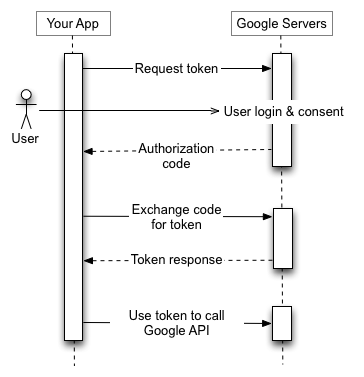
\includegraphics[width = 0.5\textwidth]{Imagenes/Bitmap/webflow.png}%
	\caption{OAuth 2.0 for Web Server Applications and Installed Applications.}%
	Image extracted from \cite{oauth}
	\label{fig:oauth}
\end{figure}

After constructing an \textit{InstalledAppFlow} by calling \textit{from\_client\_secrets\_file} as we have explained, we can invoke the class method \textit{run\_local\_server} which instructs the user to open the authorization URL in the browser and will try to automatically open it. This function will start a local web server to listen for the authorization response. Once there is a reply, the authorization server will redirect the user's browser to the local web server. As we can see in Figure \ref{fig:oauth}, the web server will get the authorization code from the response and shutdown, that code is then exchanged for a token.

Then, we will be in possession of the OAuth 2.0 credentials for the user \citep{oauth2.credentials} which we are going to use for accessing the user's Gmail account. In summary, it is possible to obtain the necessary permissions from the user and to follow the OAuth 2.0 protocol, by executing these instructions (written in Python):

\begin{python}
from google_auth_oauthlib.flow import InstalledAppFlow

# Create a flow instance
flow = InstalledAppFlow.from_client_secrets_file('credentials.json', 
	['https://mail.google.com/'])
# Obtain OAuth 2.0 credentials for the user
creds = flow.run_local_server(port = 0)
\end{python}

Now, we are able to call Gmail API by using the token (which is stored in the variable \textit{creds}). However, before starting working on the email data, we should save the OAuth 2.0 credentials since otherwise the user would need to go through the consent screen every time the application is opened. To prevent the latter from happening, to differentiate access from mail management and consequently to reuse as much code as possible, we have implemented the following class \textit{auth}, in \textit{auth.py}, with a main method \textit{get\_credentials}:

\begin{pythonnum}
import pickle
import os.path
from google_auth_oauthlib.flow import InstalledAppFlow
from google.auth.transport.requests import Request
	
class auth:
	def __init__(self, SCOPES, CLIENT_SECRET_FILE):
		self.SCOPES = SCOPES
		self.CLIENT_SECRET_FILE = CLIENT_SECRET_FILE
	
	def get_credentials(self):
		"""
		Obtains valid credentials for accessing Gmail API
		"""
		creds = None
		# The file token.pickle stores the user's access and refresh tokens
		if os.path.exists('token.pickle'):
			with open('token.pickle', 'rb') as token:
				creds = pickle.load(token)
		# If there are no (valid) credentials available, let the user log in
		if not creds or not creds.valid:
			if creds and creds.expired and creds.refresh_token:
				creds.refresh(Request())
			else:
				flow = InstalledAppFlow.from_client_secrets_file(
					self.CLIENT_SECRET_FILE, self.SCOPES)
				creds = flow.run_local_server(port=0)
			# Create token.pickle and save the credentials for the next run
			with open('token.pickle', 'wb') as token:
				pickle.dump(creds, token)
		return creds

\end{pythonnum}

As we can observe in line 17 within \textit{get\_credentials} method, at first we check if the file called \textit{token.pickle} exists, and in that case, it is opened and its information is stored in the variable \textit{creds}. Thus, we avoid to force the user to open the authorization screen. By contrast, as we have seen before, if it does not exists, we obtain the credentials by calling the class methods \textit{from\_client\_secrets\_file} and \textit{run\_local\_server} (it is written between lines 25 and 30).

There is another case that is also reflected in the code above (in lines 23 and 24): the credentials are expired (it is possible to check it by executing \textit{creds.expired}) and they can be refreshed (the OAuth 2.0 refresh token is \textit{creds.refresh\_token}) \citep{oauth2.credentials}. In this situation, we will refresh the access token by invoking the method known as \textit{refresh} and by giving it a \textit{Request} object \citep{request-lib} from \textit{google.auth.transport.requests} as the function parameter which used to make HTTP requests.

\subsection{Building a Gmail Resource} \label{ssect:gmailres}
At this point, with the OAuth 2.0 credentials, we are able to call the Gmail API. For this purpose, it is necessary to construct a resource \citep[/v1/reference]{gmailAPI} for interacting with the API. The \textit{build} method, from \textit{googleapiclient.discovery} library \citep{build-module}, create that object. As we will see later, this resource will lead us to manage emails, drafts, threads and everything we will like to do with the user's Gmail data. This is why, using the \textit{auth.py} file explained in Section \ref{ssect:oauth}, we are going to start every user session with the instructions below (or their equivalents in the language we are using):

\begin{python}
from googleapiclient.discovery import build
import auth

SCOPES = ['https://mail.google.com/']
CLIENT_SECRET_FILE = 'credentials.json'

# Creation of an auth instance
authInst = auth.auth(SCOPES, CLIENT_SECRET_FILE)
# Constructing the resource API object
service = build('gmail', 'v1', credentials = authInst.get_credentials())
\end{python}

Henceforth, we will use the \textit{service} variable to relate it with the resource object created by the \textit{build} method.

\subsection{Users resource}\label{ssect:userres}
The \textit{build} method could be called for obtaining any resource of any Google API (by giving it the suitable parameters). Our specific created \textit{service}\footnote{\url{http://googleapis.github.io/google-api-python-client/docs/dyn/gmail\_v1.html}} has an important instance method that we are going to invoke for every execution: the \textit{users()} method. It returns what is known as users resource \citep[/v1/reference/users]{gmailAPI}.

The users resource has also instance methods, which return other Gmail API resources that we are going to need, such as \textit{drafts()} (see Section \ref{ssect:drafts}), \textit{labels()} (see Section \ref{ssect:labres}), \textit{messages()} (see Section \ref{ssect:msgres}) and \textit{threads()} (see Section \ref{ssect:threads}) which return drafts, labels, messages and threads resources respectively. Moreover, it possesses the three methods that we explain hereunder (we must remember that for being able to execute any method that we are going to explain in this and next sections, it is necessary to have the appropriate authorization with at least one of the required scopes that we can look up in its documentation):

\begin{itemize}
	\item\textit{getProfile(userId)}: it returns an object with a dictionary structure as it follows:
	\begin{python}
	{
	'threadsTotal' : integer, # Total number of threads in the mailbox
	'emailAddress' : string, # User's email address
	'historyId' : string, # ID of the mailbox's current history record
	'messagesTotal' : integer # Total number of messages in the mailbox
	}
	\end{python}
	The parameter is a string with the user's email address. If we remember the authentication process, at no time we ask the user about the email address because we decided to let the Google API functions to handle all that procedure. Therefore we have no way to know this information. Nevertheless, the special string value \textit{'me'} can be used to indicate the authenticated user. For knowing the required scopes for invoking this function look up in \cite[/v1/reference/users/getProfile]{gmailAPI}.
	\item\textit{stop(userId)}: stop receiving push notifications for the given user mailbox. As it happens with \textit{getProfile}, the parameter is a string with the user's email address, but it is possible to use the especial string value \textit{'me'}.
	\item\textit{whatch(userId, body)}: set up or update a push notification watch on the given user mailbox.
\end{itemize}

As we are going to call only the \textit{getProfile} method, we have described on details this first function and we have just given an idea about what the rest of them do. Now, in next sections, we are going to explain all the resources we can create with the user resource.

\subsection{Labels resource}\label{ssect:labres}
As we have seen in the explanation of the users resource (Section \ref{ssect:userres}), we can obtain the labels resource \citep[/v1/reference/users/labels]{gmailAPI} by invoking \textit{labels()} instance method of our users resource, that is to say, by using our \textit{service} variable, the instruction \textit{service.users().labels()} will return the label resource.

Thanks to labels we are able to categorize messages and threads within the user's mailbox. They have a dictionary structure and their representation is what we can observe hereunder:

\begin{python}
{
'id' : string, # The immutable identifier of the label
'name' : string, # The display name
# The visibility of messages in the Gmail web interface
'messageListVisibility' : string,
'labelListVisibility' : string, # The visibility of label
'type' : string, # The owner type of the label ('system' or 'user')
'messagesTotal' : integer, # Total number of messages with the label
'messagesUnread' : integer, # Number of unread messages with the label
'threadsTotal' : integer, # Total number of threads with the label
'threadsUnread' : integer, # Number of unread threads with the label
'color' : {
	'textColor' : string, # Text color of the label, represented as hex string
	'backgroundColor' : string # Background color represented as hex string #RRGGBB
	}
}
\end{python}

The important fields we are going to need are the \textit{name} and the \textit{type}. Labels with \textit{system} type, such as \textit{INBOX}, \textit{SENT}, \textit{DRAFTS} and \textit{UNREAD}, are internally created and cannot be added, modified or deleted.

In order to obtain a label object, we will use the methods of this resource: create, delete, get, list, patch and update. In this manner, for example, we can store a label object by calling the next instructions:

\begin{python}
labels = service.users().labels()
labelList = labels.list(userId = 'me').execute()
label = labels.get(id = labelList[0]['id'], userId = 'me')
\end{python}

It is necessary to use the \textit{get} method because, as we can look up in \cite[/v1/reference/users/labels/list]{gmailAPI}, the \textit{list} method only contains an \textit{id}, \textit{name}, \textit{messageListVisibility}, \textit{labelListVisibility} and \textit{type} of each label, whereas the \textit{get} method returns the label resource with all the information.

\subsection{Messages resource}\label{ssect:msgres}
In most of the operations we are going to execute the correct management of messages will be essential. Therefore, knowing how the emails are represented in Gmail API and how to use them is imperative to understand how to work with this API. For this reason, in this section we are going to delve into the messages resource of the Gmail API, its structure and its methods. As we saw in Section \ref{ssect:userres}, we can access to this resource by invoking the \textit{messages()} method when we have a users resource.

\subsubsection{Resource representation}\label{sssect:msgresrep}

Regardless of which programming language is used, a messages resource \citep[/v1/reference/users/messages]{gmailAPI} internally has a dictionary structure as we can see down below:

\begin{python}
{
'id' : string,
'threadId' : string,
'labelIds' : [ string ],
'snippet' : string,
'historyId' : unsigned long,
'internalDate' : long,
'payload' : {
	'partId' : string,
	'mimeType' : string,
	'filename' : string,
	'headers' : [
		{
		'name' : string,
		'value' : string
		}
	],
	'body' : {
		'attachmentId' : string,
		'size' : integer,
		'data' : bytes
	},
	'parts' : [ (MessagePart) ]
	},
'sizeEstimate' : integer,
'raw' : bytes
}
\end{python}

The more important keys of this data structure for this work are:
\begin{itemize}
	\item\textit{id}: an immutable string which identifies the message.
	\item\textit{threadId}: we will explain the thread resource in Section \ref{ssect:threads} and we will see that a thread is composed of different messages that share common characteristics. The value of this field is a string which represent the identifier of the thread the message belongs to.
	\item\textit{labelIds}: a list of the identifiers of labels (see Section \ref{ssect:labres}) applied to the message.
	\item\textit{payload}: as we can see in the resource representation above, it has a dictionary data structure. The \textit{payload} field is the parsed email structure in the message parts. The more important keys of the \textit{payload} field are:
	\begin{itemize}
		\item\textit{mimeType}: the MIME type (see the explanation of \textit{Content-Type} header in Section \ref{sssect:mime}) of the message part.
		\item\textit{headers}: a list of headers. It contains the standard RFC 2822 \citep{rfc2822} email headers such as \textit{To}, \textit{From}, \textit{Subject} and \textit{Date}. Each header has a \textit{name} field, which is the name of the header (for example \textit{From}), and a \textit{value} field, which is the value of the header (following the same example as with the \textit{name} field: \textit{example@gmail.com} could be the value).
		\item\textit{parts}: a list which contains the different MIME message child parts (we will delve into this field in Section \ref{sssect:mime}).
		\item\textit{body}: a dictionary structure which contains the body data of this part (see Section \ref{sssect:mime}) in case it does not contain MIME message parts (otherwise it will be empty). This structure should not be confused with an attached file. Each MIME part contains a body property regardless of MIME type of the part.
	\end{itemize}
	\item\textit{raw}: the entire email message in an RFC 2822 \citep{rfc2822} formatted and base64url (see Section \ref{sssect:base64}) encoded string.
\end{itemize}

\subsubsection{Methods}\label{sssect:msgmethods}
As any other resource, the messages resource has different methods, many of whom we are going to need in the work. We will limit ourselves to describing the methods we may need to use:

\begin{itemize}
	\item\textit{attachments()}: returns the attachments resource (for more information about this resource, that we will not explain in detail, refer to \cite[/v1/reference/users/messages/attachments]{gmailAPI}).
	\item\textit{get(userId, id, format = 'full', metadataHeaders = None)}: if successful, this method returns the requested messages resource. Its parameters are:
	\begin{itemize}
		\item\textit{id}: the identifier string of the message we are looking for.
		\item\textit{userId}: the user's email address. As it happens with the \textit{getProfile} method of the users resource (see Section \ref{ssect:userres}), the special string value \textit{'me'} can be used to indicate the authenticated user.
		\item\textit{format} (optional parameter): the format in which we want the message returned. This field can take the following punctual values: \textit{'full'} (returns the entirely email data with body content parsed in the \textit{payload} messages resource field and the \textit{raw} field is empty), \textit{'metadata'} (returns only an email message with its identifier, email headers and labels), \textit{'minimal'} (returns only an email message with its identifier and labels) and \textit{'raw'} (returns the entirely email message data with the body content in the \textit{raw} messages resource field as a base64url (see Section \ref{sssect:base64}) encoded string and the \textit{payload} field is empty).
		\item\textit{metadataHeaders} (optional parameter): it is only used when the format parameter takes the punctual value of \textit{'metadata'}. It is a string list where we have to insert the headers we want to be included.
	\end{itemize}
	For knowing the required scopes for invoking this function refer to \cite[/v1/reference/users/messages/get]{gmailAPI}.
	\item\textit{list(userId, includeSpamTrash = false, labelIds = None, maxResults = None, pageToken = None, q = None)}: returns a resource with the following structure:
	\begin{python}
		{
		'messages' : [ users.messages resource ],
		'nextPageToken' : string,
		'resultSizeEstimate' : unsigned integer
		}
	\end{python}
	As it happens with the \textit{list} method of the labels resource (see Section \ref{ssect:labres}), \textit{'messages'} list does not contain all of a message information (for obtaining the full email data we can use \textit{get} method). Each element of this list only contains the \textit{id} and \textit{threadId} field.
	
	The parameters of this method are:
	\begin{itemize}
		\item\textit{userId}: user's email address (we can use the special string value \textit{'me'}).
		\item\textit{includeSpamTrash} (optional parameter): boolean parameter which determines if it includes messages with the labels \textit{SPAM} and \textit{TRASH} in the result of the operation.
		\item\textit{labelIds} (optional parameter): it is a list which let us filter the messages by only returning emails with labels that match all of the identifiers that belong to this list.
		\item\textit{maxResults} (optional parameter): an integer which determines the maximum number of messages to return.
		\item\textit{pageToken} (optional parameter): string which specifies a page of results.
		\item\textit{q} (optional parameter): string which let us do an specific query (with the same query format as the Gmail search box) and filter the messages by only returning emails that match with it.
	\end{itemize}
	For knowing the required scopes for invoking this function refer to \cite[/v1/reference/users/messages/list]{gmailAPI}.
	\item\textit{send(userId, body = None, media\_body = None, media\_mime\_type = None)}: it sends the given message to the email addresses specified in the \textit{To}, \textit{Cc} and \textit{Bcc} headers. The first two parameters are the only ones we will use. The first (\textit{userId}) is the user's email address (we can use the special string value \textit{'me'}) and the second is the message we want to send in an RFC 2822 \citep{rfc2822} formatted. For knowing the required scopes for invoking this function refer to \cite[/v1/reference/users/messages/send]{gmailAPI}.
\end{itemize}

\subsubsection{MIME} \label{sssect:mime}
To be able to create messages and read the body of the emails, it is essential to understand what the MIME standard consists of. Hence, in this section we are going to give a general idea about this.

MIME, whose acronym stands for Multipurpose Internet Mail Extensions \citep{wikimime, rfc2045}, is an Internet standard for the exchange of several file types (text, audio, video, etc.) which provides support to text with characters other than ASCII, non-text attachments, body messages with numerous parts (known as multi-part messages) and headers information with characters other than ASCII. Each data type has a different name in MIME. These names follow the format: type/subtype (both type and subtype are strings), in such a way that the first denotes the general data category and the second the specific type of that information. The values the type can take are:

\begin{itemize}
	\item\textit{text}: means that the content is simple text. Subtypes like \textit{html}, \textit{xml} and \textit{plain} can follow this type.
	\item\textit{multipart}: indicates that the message has numerous parts with independent data. Subtypes like \textit{form-data} and \textit{digest} can follow this type.
	\item\textit{message}: it is used to encapsulate an existing message, for example when we want to reply a email and add the previous message. Subtypes like \textit{partial} and \textit{rfc822} can follow this type.
	\item\textit{image}: means that the content is an image. Subtypes like \textit{png}, \textit{jpeg} and \textit{gif} can follow this type.
	\item\textit{audio}: indicates that the content is an audio. Subtypes like \textit{mp3} and \textit{32kadpcm} can follow this type.
	\item\textit{video}: denotes that the content is an video. Subtypes like \textit{mpeg} and \textit{avi} can follow this type.
	\item\textit{application}: it is used for application data that could be binary. Subtypes like \textit{json} and \textit{pdf} can follow this type.
	\item\textit{font}: means that the content is a file which defines a font format. Subtypes like \textit{woff} and \textit{ttf} can follow this type.
\end{itemize}

MIME has several headers which appear in all emails sent with this standard. The most important of them are the following:

\begin{itemize}
	\item\textit{Content-Type}: the value of this header is the type and subtype of the message with the same structure that we have explained before. For example, if we have the header \textit{Content-Type: text/plain}, it means that the message is a plain text. By using the type \textit{multipart} make the creation of messages with parts and subparts organized in a tree structure (in which leaf nodes can belong to any type and the rest of them can belong to any multipart subtype variety) possible \citep[Section 7.2]{rfc1341}. A feasible composition of a message with a part with plain text and other non-text parts could be constructed by using \textit{multipart/mixed} as the root node like in Figure \ref{fig:content-type}. Indeed, in the example of Figure \ref{fig:content-type}, we can observe the use of \textit{multipart/alternative} for a message which contains the body both in plain text and in html text. Other different emails constructions are possible (like forwarding with the original message attached by using \textit{multipart/mixed} with a \textit{text/plain} part and a \textit{message/rfc822} part) thanks to the tree structure of the \textit{Content-type} header.
	
	Another important detail, that we can observe in the example in figure \ref{fig:content-type}, is the fact that each node of the tree structure of the emails is visited and showed following the pre-order traversal.
	
	\begin{figure}[t]
		\centering%
		\includegraphics[width = 1.2\textwidth]{Imagenes/Bitmap/tree-content-type.png}%
		\caption{MIME types tree structure of an email example}%
		\label{fig:content-type}
	\end{figure}
	\item\textit{Content-Disposition}: this header is used to indicate the presentation style of the part of the message. There are two ways to show the part: \textit{inline} content-disposition (which means that the content must be displayed at the same time as the message) and \textit{attachment} content-disposition (the part is not displayed at the same time as the message and it requires some form or action from the user to see it). Furthermore, this header also provides several fields for specifying other type of information about the content, such as the name of the file and the creation or modification date. The following example is taken from RFC 2183 \citep{rfc2183} and, as we will explain after the example, it does not match with the syntax of this same header in the example that we can see in the last part of the example message of figure \ref{fig:content-type}:
	\begin{lstlisting}
		Content-Disposition: attachment; filename=genome.jpeg;
			modification-date="Wed, 12 Feb 1997 16:29:51 -0500";
	\end{lstlisting}
	As we have said, this syntax is different from the used in the email example of Figure \ref{fig:content-type}. This results from the fact that, in HTTP, the header we find in that figure (\textit{Content-Disposition: attachment}) is usually used for instructing the client to show the response body as a downloadable file. As we can observe, it has a \textit{filename} field which is used for establishing the default file name when the user is going to download it.
	
	\item\textit{Content-Transfer-Encoding}: when we want to send some files in a message, sometimes they are represented as 8-bit character or binary data, which are not allowed in some protocols. On this account, it is necessary to have a standard that indicates how we should re-encoding such data into a 7-bit short-line format. The Content-Transfer-Encoding header \citep[Section 5]{rfc1341} will tell the client which transformation has been used for being able to transport that data. Therefore and for lack of a previous standard which states a single Content-Transfer-Encoding mechanism, the possible values, which specify the type of encoding are: \textit{'base64'} (see Section \ref{sssect:base64}), \textit{'quoted-printable'} (see Section \ref{sssect:quot-p}), \textit{'8bit'}, \textit{'7bit'}, \textit{'binary'} and \textit{'x-token'}. All these values are not case sensitive. If this header does not exist, we can assume that the value of this header is \textit{'7bit'}, which means that the body of the message is already in a seven-bit mail-ready representation, in other words, all the body of the message is represented as short lines of US-ASCII data. Despite the \textit{'8bit'}, \textit{'7bit'} and \textit{'binary'} indicate that the content has not been transformed, they are useful for knowing the kind of encoding that the data has. This header will generally be omitted when the Content-Type has the \textit{multipart} or \textit{'message'} type (as it happens in the message example of Figure \ref{fig:content-type}), because it also admits the last three types we have mentioned.
	
	It is common to add another header (as we can see in Figure \ref{fig:content-type}) called \textit{charset}, which value represents the original encoding of data so the client is able to decode it.
\end{itemize}

\subsubsection{Base64} \label{sssect:base64}
As we have seen, in the field \textit{raw} of the messages resource (see Section \ref{sssect:msgresrep}) the entire email message has to be encoded using base64url; and, as we have studied when we learnt how the MIME standard (see Section \ref{sssect:mime}) is, we can find email whose content encoding is base64. Base64 \citep{wikibase64, rfc4648} is a group of reversible binary-to-text encoding schemes which represent binary data as a sequence of ASCII printable characters. It makes use of a radix-64 to translate each character, because 64 is the higher power of two than can be represented using only printable ASCII characters. Indeed all the Base64 variants (like base64url) utilise the characters range A-Z, a-z and 0-9 in that order for the first 62 digits, but the chosen symbol for the last two digits are very different between them. In particular, the MIME (see Section \ref{sssect:mime}) specification, established in RFC 2045 \citep{rfc2045}, describes base64 based on  Privacy-enhanced Electronic Mail (PEM) protocol \citep{wikipem, rfc7468}, which means that the last two characters are '+' and '/' and the symbol '=' is used for output padding suffix. In the same way, MIME does not stablish a fixed size for the base64 encoded lines, by contrast it specifies a maximum size of 76 characters.

If we try to apply standard base64 in a URL encoder, it will translate the characters '+' and '/' to its hexadecimal representation ('+' = '\%2B' y '/' = '\%2F'). This will cause a conflict in heterogeneous systems or if we use it in data base storage, because of the character '\%' produced by the encoder (it is a special symbol of ANSI SQL). This is why modified Base64 for URL variants exists (such as base64url in \cite{rfc4648}), where the '=' character has no usefulness and the '+' and '/' symbols are replaced by '-' and '\_' respectively. Besides it has no impact on the size of encoded lines.

\subsubsection{Quoted-printable} \label{sssect:quot-p}
Other reversible binary-to-text encoding that could be used in the content of a MIME message is the quoted-printable encoding \citep{wikiquotprint, rfc1521}. Making use of printable characters (such as alphanumeric and '=') proved capable of transmitting 8 bit data over a 7 bit protocol. Unlike base64, if the original message is mostly composed of ASCII characters, the encoded text is readable and compact.

Each byte could be represented via two hexadecimal character. On this basis, the '=' symbol followed by two hexadecimal digits are enough to encode all the characters except the printable ASCII ones and the end of line. For example, if we want to represent the 12th ASCII character we can encode it as '=0C' or if the equality symbol (whose decimal value is 61) is in our original message, it could be encoded as '=3D' (note that despite being a printable ascii character it must be encoded as it is a special character in this encoding). This is how quoted-printable encodes the different characters.

In respect of the maximum line size, as it happens with the MIME specification of the base64 (see Section \ref{sssect:base64}), it is 76 characters each encoded line. To achieve this goal and still be able to decode the text getting the original message, quoted-printable adds \textit{soft line breaks} at the end of the line consisting of the '=' symbol and it does not modify the encoded text.

\subsection{Threads resource}\label{ssect:threads}
When we access to our inbox, we are actually seeing the inbox threads instead of the messages resource. Every message, even if it is an only email without a reply, is enclosed in a thread resource \citep[/v1/reference/users/threads]{gmailAPI} which is essentially a list, perhaps unitary, of messages resources. In fact, as we can observe in the following resource representation, in its dictionary structure it has a list of messages resources:

\begin{python}
	{
		'id' : string, # The identifier of the thread
		'snippet' : string, # A short part of the text
		'historyId' : unsigned long,
		'messages' : [ users.messages resource ]
	}
\end{python}

The most important methods of this resource are:
\begin{itemize}
	\item\textit{get(userId, id, format = 'full', metadataHeaders = None)}: if successful, this method returns the requested threads resource. In respect of the parameters, they are defined in the same way as in \textit{get} messages resource method (see Section \ref{sssect:msgmethods}) with the exception of the parameter \textit{format}, whose only difference is that it does not accept the \textit{'raw'} value. For knowing the required scopes for invoking this function look up in \cite[/v1/reference/users/threads/get]{gmailAPI}.
	\item\textit{list(userId, includeSpamTrash = False, labelIds = None, maxResults = None, pageToken = None, q = None)}: if successful, it returns a dictionary structure analogous to the view in the \textit{list} message resource method (see Section \ref{sssect:msgmethods}). Needless to say, instead of returning a messages resource list it will give us a threads resource list, which does not contain the complete information of each thread (for example each element of the list has not a list of messages resource). Full thread data can be fetched using the previous method. The parameters of this method are defined in the same way as the \textit{list} messages resource method. For knowing the required scopes for invoking this function refer to \cite[/v1/reference/users/threads/list]{gmailAPI}.
\end{itemize}

\subsection{Drafts resource}\label{ssect:drafts}
The last Gmail API resource we will study is the most easy to understand after knowing all the structures related with emails that we have explained in the above sections: the drafts resource \citep[/v1/reference/users/drafts]{gmailAPI}. Its representation is very simple:

\begin{python}
	{
		'id' : string # The immutable identifier of the draft
		'message' : users.messages resource
	}
\end{python}

As we can observe, a draft is virtually a messages resource with an identifier. Indeed, in order to create a new draft with the \textit{DRAFT} label we must create a MIME message (see Section \ref{sssect:mime}) as we have to do when we want to send a new email by using the \textit{send} messages resource method. Then it is necessary to invoke the drafts resource method \textit{create(userId, body = None, media\_body = None, media\_mime\_type = None)} by giving the value \textit{'me'} and the message created to the first to parameters.

\subsection{API Usage Limits} \label{ssect:apilimits}
One factor to be taken into account is the limitations of the Gmail API \citep[/v1/reference/quota]{gmailAPI} which could become a drawback in the application development. It has a limit on the daily usage and on the per-user rate. In order to measure the usage rate, ``quota units'' are defined depending on the method invoked. In Table \ref{tab:quotaUnits} we can consult the value of some methods in quota units (we have selected the more important methods for our purpose, for the quota units of other methods it is recommended to refer to \cite[/v1/reference/quota]{gmailAPI}).

\begin{table}[h]
	\centering
	\begin{tabular}{|l c r|}
		\hline
		\textbf{Method} & \textbf{Section where the method is explained} & \textbf{Quota units} \\
		\hline\hline
		\textit{getProfile} & \ref{ssect:userres} & 1\\ \hline
		\textit{labels.get} & \ref{ssect:labres} & 1\\ \hline
		\textit{messages.get} & \ref{sssect:msgmethods} & 5\\ \hline
		\textit{messages.list} & \ref{sssect:msgmethods} & 5\\ \hline
		\textit{messages.send} & \ref{sssect:msgmethods} & 100\\ \hline
		\textit{threads.get} & \ref{ssect:threads} & 10\\ \hline
		\textit{threads.list} & \ref{ssect:threads} & 10\\ \hline
		\textit{drafts.create} & \ref{ssect:drafts} & 10\\ \hline
	\end{tabular}
	\caption{Main methods' quota units}
	\label{tab:quotaUnits}
\end{table}

However, both daily usage limit and per-user rate limit are acceptable for the type of software we want to build: 1,000,000,000 quota units per day and 250 quota units per user per second. Therefore there are no constraints (for our purpose) that avoid us to use this API.


\section{Electronic Mail Protocols}
Apart from Gmail API (see section \ref{sect:gmailapi}), there is another way to read, send emails and access to the user's email data and this is by directly using the communication protocol for electronic mail transmission and the internet standard protocol to retrieve email messages from a mail server over a TCP/IP connection. In this section we are going to study the main email management protocols, both electronic mail transmission protocol (such as Simple Mail Transfer Protocol, which is explained in section \ref{ssect:smtp}) and message access protocol (such as Internet Message Access Protocol and Post Office Protocol, which are studied in sections \ref{ssect:imap} and \ref{ssect:pop}, respectively).

In spite of being a mail server-independent solution, as we will see, we are going to find security issues which are going to hinder our user's email data access. These trials come from the automatic server access. The assessment of the advantages and disadvantages of making use of the email protocols or the Gmail API is discussed in section \ref{ssect:protvsapi}.

\subsection{Simple Mail Transfer Protocol} \label{ssect:smtp}

Simple Mail Transfer Protocol (also known as SMTP) is a network connection-oriented communication protocol used for the exchange of e-mail messages. It was originally defined in \cite{rfc821} (for the transfer) and in \cite{rfc822} (for the message). It is currently defined in \cite{rfc5321} and \cite{rfc5322}. However, this protocol has some limitations when it comes to receiving messages on the destination server. For this reason, this task is intended for other protocols such as the Internet Message Access Protocol (see section \ref{ssect:imap}) or the Post Office Protocol (refer to point \ref{ssect:pop}), and SMTP is used specifically to send messages.

Making use of SMTP, mail is ``pushed'' from one mail server to another (next-hop mail server) until it reaches its destination. The message is not routed according to the message recipients specified during the client's connection to the SMTP server, but from the destination mail server. Thanks to the fact that this protocol has a feature to initiate mail queue processing, intermittently connected mail server can extract messages from another remote server when necessary.

\subsection{Post Office Protocol} \label{ssect:pop}

Post Office Protocol (also known as POP) is an application protocol (in OSI Model) for obtaining e-mails stored in a remote Internet server called POP server. It was originally defined in \cite{rfc918} (it was POP version 1, also known as POP1). Current POP version (POP3, in general when we talk about pop we refer to this version) is detailed in \cite{rfc1939}.

POP was designed for receiving emails. Using POP, users with intermittent or very slow Internet connections (such as modem connections) can download their email while online and check it later even when offline. The general operation is: a client using POP3 connects, gets all messages, stores them on the user's computer as new messages, deletes them from the server, and finally disconnects. However some mail clients include the option to leave messages on the server. They use the order UIDL (Unique IDentification Listing) which, unlike most POP3 commands, does not identify messages depending on their mail server ordinal number, due to the fact that this creates problems when a client tries to leave messages on the server, since messages with numbers change from one connection to the server to another. Accordingly, server which makes use of UIDL, assigns a unique and permanent character string to each message. Thus, when a POP3-compatible mail client connects to the server, it uses the UIDL command to map the message identifier. This way the client can use that mapping to determine which messages to download and which to save at the time of download.

Like other old Internet protocols, POP3 used a signature mechanism without encryption. The transmission of POP3 passwords in plain text still occurs. Nowadays POP3 has various authentication methods that offer a diverse range of levels of protection against illegal access to users' mailboxes.

The advantage over other protocols is that between server-client you don't have to send so many commands for communication between them. The POP protocol also works properly if you do not use a constant connection to the Internet or to the network that contains the mail server.

\subsection{Internet Message Access Protocol} \label{ssect:imap}

Internet Message Access Protocol (also known as IMAP) is an application protocol, designed as an alternative to Post Office Protocol (se section \ref{ssect:pop}) in 1986, which allows the access to stored messages in an Internet server. As with the Post Office Protocol, with IMAP you can access your e-mail from any computer with an Internet connection. The current version of IMAP (IMAP version 4 review 1 or IMAP4rev1) is defined in \cite{rfc3501}.

In contrast to Post Office Protocol, IMAP allows multiple clients to manage the same mailbox. This fact results from the main difference between these two protocols: IMAP does not remove email from server until the client specifically requests it and it does not download the messages to the user's computer (clients may store a local copy of them, but these are considered to be temporary data).

\subsection{Advantages and disadvantages of email protocols versus the use of Gmail API} \label{ssect:protvsapi}
